\documentclass[10pt,a4paper]{article}
\usepackage[utf8]{inputenc}
\usepackage[czech]{babel}
\usepackage[T1]{fontenc}
\usepackage{amsmath}
\usepackage{amsfonts}
\usepackage{amssymb}
\usepackage{graphicx}
\usepackage{caption}
\usepackage{subcaption}
\usepackage{placeins}
\usepackage{url}
\usepackage{multirow}
\usepackage[left=2cm,right=2cm,top=3cm,bottom=3cm]{geometry}

\title{Závěrečná zpráva k projektu z Neuronových sítí}
\author{Marie Drábková, Jiří Novotný, Jakub Peschel}


\begin{document}
\maketitle

\section*{Úvod}
Našim cílem je vytvořit neuronovou síť, která rozpoznává, kdo vyhrál v piškvorkách $3\times 3$. Vstupem sítě je finální konfigurace hrací plochy (dále endgame). Výstupem je klasifikace, zda vyhrál  \uv{křížek}, \uv{kolečko} nebo hra skončila remízou. 

Cíl jsme si rozdělili do tří fází. V poslední fázi by síť měla ideálně klasifikovat bitmapový obrázek hrací plochy.


\subsection*{Data}
Téma práce je inspirováno databází UCI Machine Learning \footnote{\url{https://archive.ics.uci.edu/ml/datasets/Tic-Tac-Toe+Endgame}}, ale my jsme se rozhodli klasifikovat i případy výhry \uv{kolečka} a remízy, které databáze nezahrnovala. Proto jsme si vytvořili vlastní generátor endgames v textovém formátu. Dále jsme vytvořili konvertor textových dat do bitmapových obrázků.

Existuje celkem 958 možných endgames. Z nich v 626 případech vyhrál X, v 316 vyhrál O a v 16 hra skončila remízou. Základní data představuje rozdělení do tréninkových, validačních a testovacích množin v poměru 60:20:20 tak, že v každé množině je stejné procentuální zastoupení vítězství X, O a remíz. Dále jsme data různým způsobem modifikovali, což bude popsáno níže.

\section*{Implementace}
TODO Jirka: epocha, batchsize, rychlost učení, inicializace vah, chybová funkce, sigmoida, velikost sítě, proč vícevrstvá síť


\section*{Učení}
\subsection*{Textový vstup}
Nejdřív jsme síť naučili na jednoduchém textovém vstupu, který představuje dvourozměrné pole $3\times 3$. Jeho prvky jsou hodnoty z množiny $\{-1,0,1\}$, které reprezentují  postupně \uv{kolečko}, prázdné pole a \uv{křížek}.

Jako první jsme vyzkoušeli velikost sítě (9,9,3), rychlost učení 0,05, 500 epoch. Síť se naučila rozpoznávat hry s přesností 98,4\,\% za cca 60 epoch. Dále byla přesnost stabilní. Ačkoliv cost function nadále klesala, síť se nepřeučovala, viz grafy \ref{fig:1}. Matice zmatenosti \ref{mz1} (R znamená remíza) ukazuje, že se síť dobře rozpoznává vítězství X a O, ale má problém poznat remízu, protože v tréninkových datech se konfigurace znamenající remízu vyskytují příliš málo a síť se je nezvládne naučit. 

\begin{figure}[h!]
\centering
\begin{subfigure}{.5\textwidth}
  \centering
  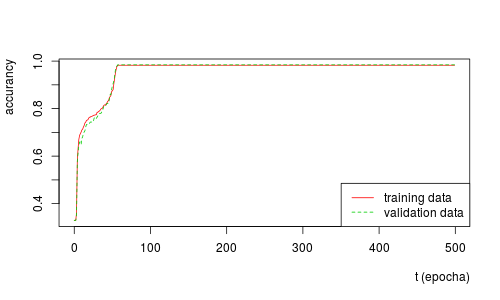
\includegraphics[width=\textwidth]{a1}
  \caption{Accurancy}
  \label{fig:a1}
\end{subfigure}%
\begin{subfigure}{.5\textwidth}
  \centering
  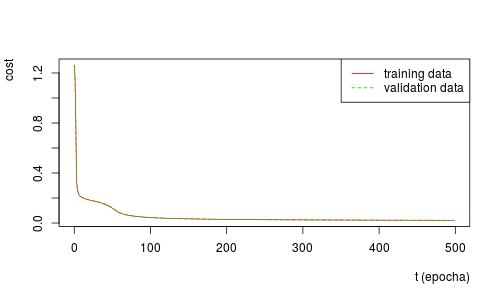
\includegraphics[width=\textwidth]{c1}
  \caption{Cost}
  \label{fig:c1}
\end{subfigure}
\caption{Textový vstup, síť (9,9,3)}
\label{fig:1}
\end{figure}


\shorthandoff{-}
\begin{table}[h!]
\centering
\begin{tabular}{|c|c|c|c|c|}
\hline 
& \multicolumn{4}{c|}{Actual} \\ \cline{2-5}
& & X& O & R\\\hline 
\multirow{3}*{Predicted}& X & 125 & 0 & 3 \\ \cline{2-5}
& O & 0 & 63 & 0 \\ \cline{2-5}
& R &0 & 0 & 0 \\ \hline 
\end{tabular}
\shorthandon{-}
\caption{Matice zmatenosti pro síť (9,9,3) a textový vstup}
\label{mz1}
\end{table}

\FloatBarrier
Poté jsme postupně zkoušeli zmenšovat velikost sítě na (9,3,3) až (9,3). I síť bez vnitřní vrstvy byla schopna dávat stejné výsledky jako výše popsaná síť (9,9,3). Pouze průběh učení byl jiný, viz grafy \ref{fig:2}. Matice zmatenosti vypadá stejně, viz \ref{mz1}. 







\begin{figure}[h!]
\centering
\begin{subfigure}{.5\textwidth}
  \centering
  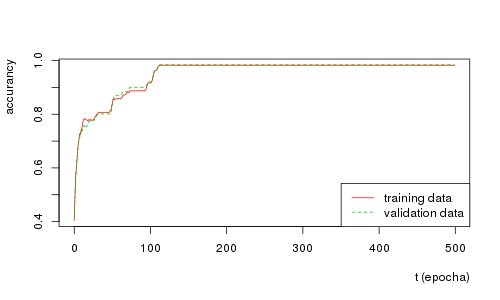
\includegraphics[width=\textwidth]{a2}
  \caption{Accurancy}
  \label{fig:a2}
\end{subfigure}%
\begin{subfigure}{.5\textwidth}
  \centering
  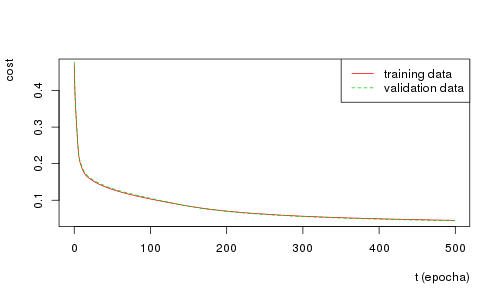
\includegraphics[width=\textwidth]{c2}
  \caption{Cost}
  \label{fig:c2}
\end{subfigure}
\caption{Textový vstup, síť (9,3)}
\label{fig:2}
\end{figure}


Po podrobnějším zkoumání vah jsme dospěli k závěru, že síť považuje za výherce X právě tehdy, když suma na hrací ploše je 1 a pokud je suma 0, považuje za výherce O. Jenomže pokud hrací plocha představuje remízu, suma je taky jedna a síť tuto situaci klasifikuje jako výhru X.

\subsubsection*{Pokus o řešení špatně interpretovaných remíz}\label{dupl}
Nejdříve jsme chtěli síti umožnit větší šanci pro naučení remízových stavů, a proto jsme zduplikovali remízové endgames v tréninkové množině (dále duplikovaná data). Tato data jsme použili pro trénink sítě velikosti (9,3), ale nic nového se nenaučila. 

Větší síť (9,9,3) zvýšila svou přesnost na testovací množině z 98,4\,\% na 99,5\,\%. Z matice zmatenosti \ref{mz2} je vidět, že některé případy remízy dokážeme rozpoznat. Pro ilustraci uvádíme tabulky zmatenosti trénovací (tabulka \ref{mz3} i validační (tabulka \ref{mz4}) množiny při celkové přesnosti na testovacích datech 99,5\,\%.

Pak jsme zmenšili rychlost učení z 0,05 na 0,01 a zvětšili počet epoch z 500 na 1000. Touto úpravou jsme dosáhli přesnosti 100\,\% na testovacích datech, ale tento výsledek není stabilní. Při replikaci pokusu jsme dosahovali různých výsledků mezi 97\,\% a 100\,\%.  

\shorthandoff{-}
\begin{table}[h]
\centering
\begin{tabular}{|c|c|c|c|c|}
\hline 
& \multicolumn{4}{c|}{Actual} \\ \cline{2-5}
& & X& O & R\\\hline 
\multirow{3}*{Predicted}& X & 125 & 0 & 1 \\ \cline{2-5}
& O & 0 & 63 & 0 \\ \cline{2-5}
& R &0 & 0 & 2 \\ \hline 
\end{tabular}
\shorthandon{-}
\caption{Matice zmatenosti pro síť (9,9,3) a textový vstup s opakováním na tréninkové množině}
\label{mz2}
\end{table}

\shorthandoff{-}
\begin{table}[h]
\centering
\begin{tabular}{|c|c|c|c|c|}
\hline 
& \multicolumn{4}{c|}{Actual} \\ \cline{2-5}
& & X& O & R\\\hline 
\multirow{3}*{Predicted}& X & 374 & 0 & 0 \\ \cline{2-5}
& O & 0 & 190 & 0 \\ \cline{2-5}
& R &2 & 0 & 270 \\ \hline 
\end{tabular}
\shorthandon{-}
\caption{Matice zmatenosti trénovací množiny pro síť (9,9,3) a textový vstup s opakováním na tréninkové množině}
\label{mz3}
\end{table}

\shorthandoff{-}
\begin{table}[h]
\centering
\begin{tabular}{|c|c|c|c|c|}
\hline 
& \multicolumn{4}{c|}{Actual} \\ \cline{2-5}
& & X& O & R\\\hline 
\multirow{3}*{Predicted}& X & 125 & 0 & 2 \\ \cline{2-5}
& O & 0 & 63 & 0 \\ \cline{2-5}
& R &0 & 0 & 1 \\ \hline 
\end{tabular}
\shorthandon{-}
\caption{Matice zmatenosti validační množiny pro síť (9,9,3) a textový vstup s opakováním na tréninkové množině}
\label{mz4}
\end{table}



\FloatBarrier
\subsection*{Grafický vstup $11\times 11$}
V druhé fázi jsme síti předhodili černobílý bitmapový obrázek o velikosti $11\times 11$ pixelů (viz obrázek \ref{fig:v1}). Na základních datech je výsledek stejný jako v případě textového vstupu, síť nerozpoznává remízu.

Hráli jsme si s různým nastavením sítě, ale přesnost se nijak nezlepšovala. Nejlepšího výsledku jsme dosáhli použitím duplikovaných dat popsaných v předchozí sekci a dosáhli tak přesnosti 95,5\,\%, viz grafy \ref{fig:3}.

Mezi neúspěšné pokusy patří např.:
\begin{itemize}
\item Vyrovnali jsme množství jednotlivých kategorií. Tzn. vzali z trénovací množiny 300 výher X a zbytek znásobili, aby i počet výher O a remíz byl 300.
\item Přidali jsme data tak, že jsme původní data rozšířili o konfigurace takové, kde jsme v původních datech zaměnili X a O. Prakticky to znamená přidání endgames, kdy začínal O.
\end{itemize}

\begin{figure}[h!]
\centering
\begin{subfigure}{.5\textwidth}
  \centering
  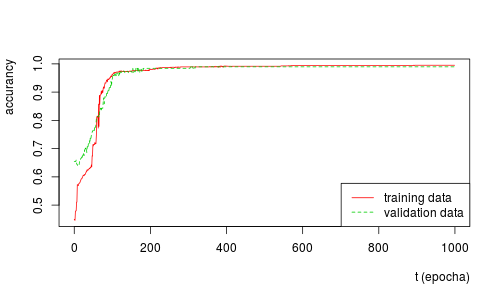
\includegraphics[width=\textwidth]{a3}
  \caption{Accurancy}
  \label{fig:a3}
\end{subfigure}%
\begin{subfigure}{.5\textwidth}
  \centering
  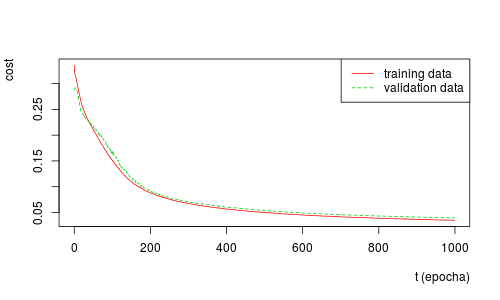
\includegraphics[width=\textwidth]{c3}
  \caption{Cost}
  \label{fig:c3}
\end{subfigure}
\caption{Grafický vstup $11\times 11$, síť (121,9,3), duplikovaná data}
\label{fig:3}
\end{figure}

\FloatBarrier
\subsection*{Grafický vstup $14\times 14$}
Dále jsme se rozhodli vyzkoušet síť na složitějším vstupu, kdy křížek nebo kolečko o velikosti $3\times 3$ pixely vkládáme náhodně do políčka o velikosti $4\times 4$ pixely, viz obrázek \ref{fig:v2}, což nám dává víc obrázků pro jeden endgame.
I síť (196,3) dává na základních datech stále stejný výsledek jako textová síť, tedy přesnost 98,4\,\% kvůli nerozpoznávání remíz. 

TODO duplikovaná data
Použitím duplikovaných dat se přesnost zvýšila na



\begin{figure}[h!]
\centering
\begin{subfigure}{.5\textwidth}
  \centering
  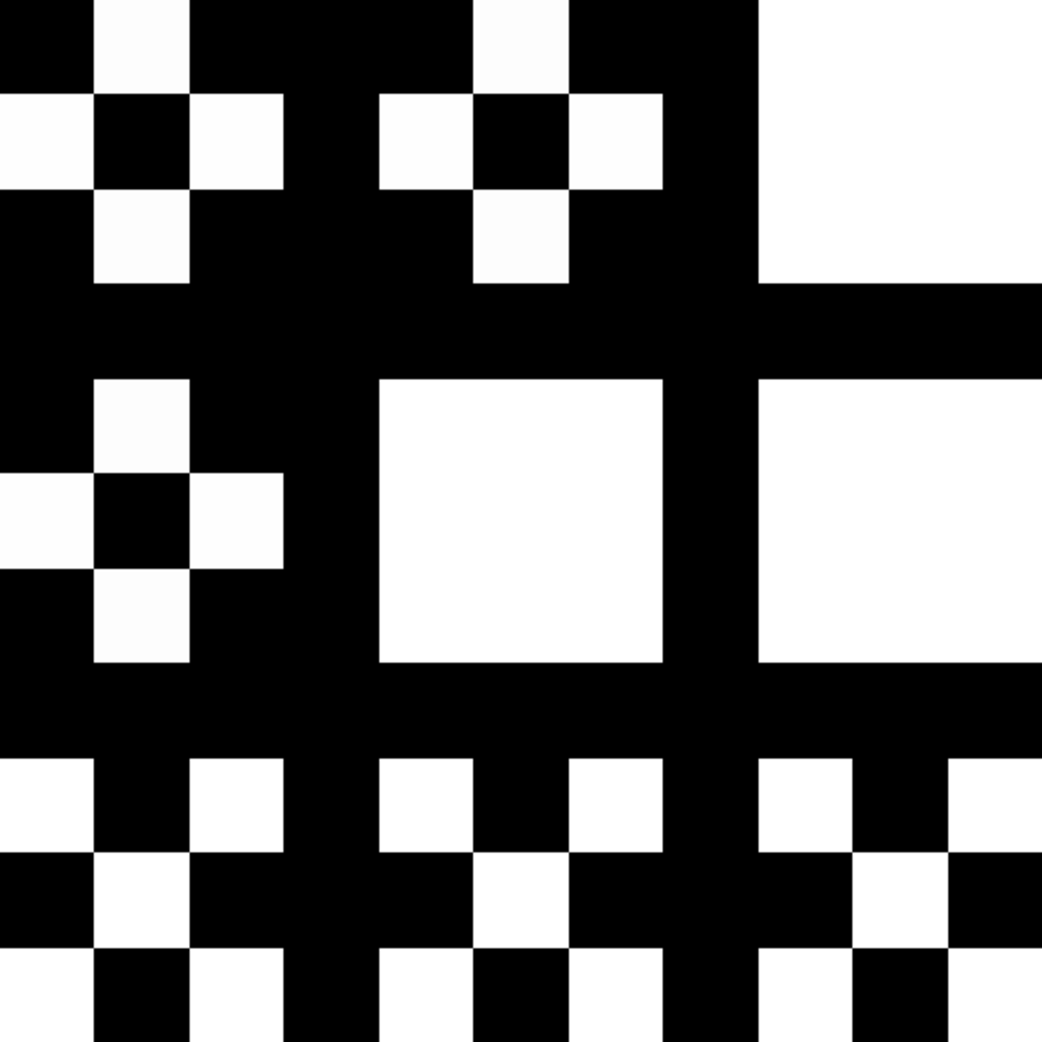
\includegraphics[scale=0.1]{vzor11}
  \caption{$11\times 11$}
  \label{fig:v1}
\end{subfigure}%
\begin{subfigure}{.5\textwidth}
  \centering
  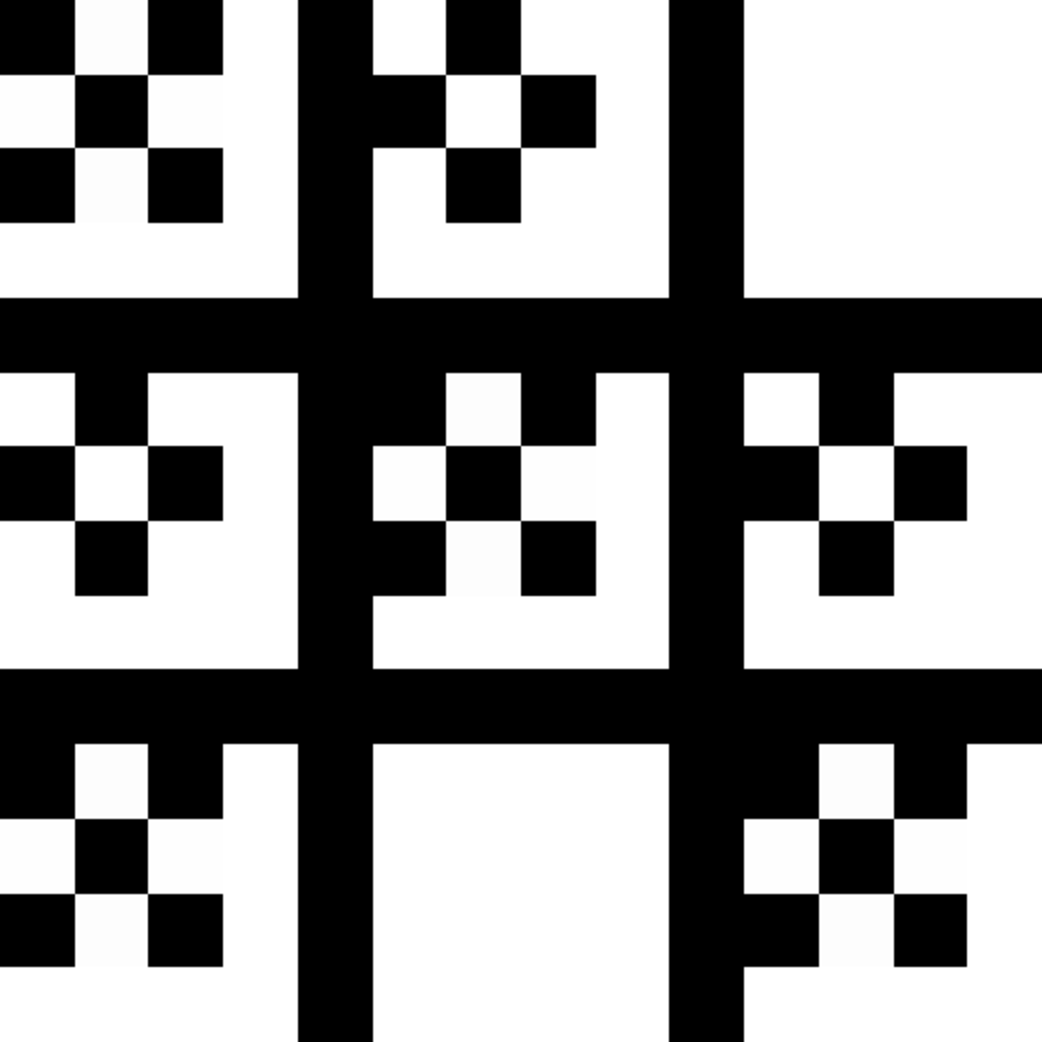
\includegraphics[scale=0.1]{vzor14}
  \caption{$14\times 14$}
  \label{fig:v2}
\end{subfigure}
\caption{Vzorový grafický vstup}
\label{fig:v}
\end{figure}

\FloatBarrier
\section*{Přínosy členů týmu}
Marie Drábková vytvořila generátor endgames a zabývala se rozdělením dat do tréninkových, validačních a testovacích množin. 
Jiří Novotný se postaral o vlastní implementaci sítě.
Jakub Peschel vytvořil konvertor textových dat do bitmapových obrázků.
Učení sítě jsme prováděli společně ve skupině.
Závěrečnou zprávu napsali Jiří Novotný a Marie Drábková.

\section*{Závěr}
Snažili jsme se vytvořit klasifikátor výherce piškvorek. Vytvořili jsme obecnou implementaci vícevrstvé neuronové sítě, generátor endgames a konvertor do bitmapových obrázků. 

Síť jsme nejprve učili na textových datech, kde jsme úpravou dat dosáhli nejlepší přesnosti 99,5\,\%, avšak síť má problémy s rozpoznáváním rozlišováním výhry X a remízy. 

Dále jsme síť učili na grafickém vstupu $11\times 11$ pixelů. 
Dosáhli jsme stejného výsledku 99,5\,\%.

TODO 14*14

Výsledné neuronové sítě neměli problém s interpretací vstupu, jak textového, tak grafického. Největším problémem bylo odlišení remíz od výher X, ale i tak síť dosahuje dobrých výsledků, protože se plete pouze v jednotkách případů. 

Použití vícevrstvé sítě pro řešení problému piškvorek zřejmě není nejvhodnější řešení, protože zanedbává prostorové rozložení dat. Domníváme se, že by bylo vhodnější použít konvoluční síť.

\end{document}